\documentclass[a4paper,12pt]{article}

% Pacotes fundamentais
\usepackage[brazil]{babel}
\usepackage[utf8]{inputenc}
\usepackage[T1]{fontenc}
\usepackage{geometry}
\usepackage{indentfirst}
\usepackage{graphicx}
\usepackage{booktabs}
\usepackage{array}
\usepackage{adjustbox}
\usepackage{float}
\usepackage{xcolor}
\usepackage{hyperref}
\usepackage{longtable}
\usepackage{amsmath}
\usepackage{amssymb}

% Configuracao das margens
\geometry{
    top=3cm,
    bottom=2cm,
    left=3cm,
    right=2cm
}

% Configuracao de hyperlinks
\hypersetup{
    colorlinks=true,
    linkcolor=blue,
    citecolor=blue,
    urlcolor=blue
}

\begin{document}

% --- CAPA ---
\begin{center}
    MINISTÉRIO DA DEFESA\\
    EXÉRCITO BRASILEIRO\\
    DEPARTAMENTO DE CIÊNCIA E TECNOLOGIA\\
    \textbf{INSTITUTO MILITAR DE ENGENHARIA}\\
    (Real Academia de Artilharia, Fortificação e Desenho -- 1792)\\[1.5cm]

    Programa Institucional de Bolsas de Iniciação em Desenvolvimento\\
    Tecnológico e Inovação (PIBITI)\\[0.4cm]
    Edital 2025/2026\\[0.8cm]

    \textbf{\large RELATÓRIO FINAL}\\[1.5cm]

    \textbf{\large Adaptação e comparação de algoritmos para o problema\\
    de roteamento de veículos utilizando programação em Julia}\\[1cm]

    Projeto: Pesquisa Operacional: Aplicação na Logística Militar\\[2cm]

    Rio de Janeiro, RJ\\
    Julho de 2026
\end{center}

\newpage

% --- IDENTIFICACAO ---
\section*{Identificação}

\begin{table}[H]
    \begin{tabular}{@{}p{4.5cm}p{10cm}@{}}
        \textbf{Autor:} & Rafael Vargas Carvalheira \\
        \textbf{E-mail:} & rafaelvargascar20@gmail.com \\
        \textbf{Telefone:} & (12) 98141-8480 \\[0.3cm]
        \textbf{Orientador:} & Prof. Orivalde Soares da Silva Júnior -- D.Sc. \\
        \textbf{E-mail:} & orivalde@ime.eb.br \\
        \textbf{Telefone:} & (21) 99939-8145 \\[0.3cm]
        \textbf{Instituição:} & Instituto Militar de Engenharia \\
        \textbf{Endereço:} & Praça Gen Tibúrcio, nr 80, Praia Vermelha -- Urca
                             (CEP: 22290-270) \\
        \textbf{Telefone:} & (21) 2546-7198 \\
        \textbf{E-mail:} & pibiti@ime.eb.br \\
    \end{tabular}
\end{table}

\newpage
\tableofcontents
\newpage

\section{Resumo}
A colaboração horizontal entre transportadoras que atendem clientes em comum permite reduzir de forma expressiva o custo agregado de transporte. Este trabalho trata do \textit{Shared Customer Collaboration Vehicle Routing Problem with Simultaneous Pickup and Delivery} (SCCVRPSPD), extensão do problema de roteamento colaborativo com clientes compartilhados na qual cada cliente possui, simultaneamente, demanda de entrega e de coleta. O modelo exato, formulado em programação linear inteira mista e resolvido com o otimizador Gurobi, não converge dentro de limites de tempo praticáveis à medida que o número de clientes cresce, o que inviabiliza seu uso operacional. Desenvolveu-se, portanto, um serviço web em Java (Spring Boot) que expõe uma meta-heurística baseada no esquema \textit{Ruin-and-Recreate}, implementada com a biblioteca Jsprit, capaz de resolver quatro cenários do problema: com e sem a restrição de simultaneidade, cada qual com e sem colaboração entre as transportadoras. A validação empregou 112 instâncias adaptadas da literatura, previamente resolvidas pelo método exato. No cenário completo, a meta-heurística apresentou diferença média de custo de 0,22\% no conjunto de 12 instâncias e de 0,36\% no conjunto de 100 instâncias, reproduzindo exatamente a solução ótima em 60 dos 100 casos e superando o incumbente do otimizador em instâncias não resolvidas até a otimalidade. O tempo de processamento manteve-se abaixo de 82 segundos em todas as execuções, contra médias superiores a 6.500 segundos do método exato nas maiores instâncias. Verificou-se ainda que a meta-heurística estima a economia proporcionada pela colaboração, de 9,50\% em média, com desvio inferior a 0,2 ponto percentual em relação ao método exato, o que a habilita como ferramenta prática de apoio à decisão.

\textbf{Palavras-chave: }roteamento de veículos; colaboração horizontal; coleta e entrega simultâneas; meta-heurística; \textit{Ruin-and-Recreate}.

\section{Apresentação}
\subsection{Introdução}
O transporte rodoviário de cargas fracionadas em áreas urbanas é realizado, em geral, por diversas empresas que operam simultaneamente sobre a mesma malha viária, partindo de centros de distribuição distintos e atendendo, com frequência, clientes localizados nas mesmas regiões. Nesse contexto, o Problema de Roteamento de Veículos (VRP, do inglês \textit{Vehicle Routing Problem}) ocupa posição central na literatura de otimização combinatória, tanto por sua relevância econômica quanto por sua dificuldade computacional, uma vez que pertence à classe dos problemas NP-difíceis.

A colaboração horizontal entre transportadoras surge como estratégia promissora de redução de custos. Quando duas empresas atendem clientes coincidentes ou muito próximos, transferir o atendimento de um cliente para a rota mais favorável da outra companhia encurta distâncias, melhora a utilização da capacidade da frota e reduz o número de veículos necessários (PAN et al., 2019; GANSTERER; HARTL, 2018). Essa vertente foi formalizada por Fernández, Roca-Riu e Speranza (2018) sob a denominação Shared Customer Collaboration \textit{Vehicle Routing Problem} (SCCVRP), no qual clientes ditos compartilhados possuem demandas junto a mais de uma transportadora e podem ser atendidos por qualquer uma delas. Extensões posteriores incorporaram janelas de tempo e limites de custo por transportadora (HIMSTEDT; MEISEL, 2021), objetivos múltiplos (ZHANG et al., 2020) e abordagens meta-heurísticas híbridas (TORRES-RAMOS et al., 2019).

Uma segunda variante relevante do VRP é a de coleta e entrega, na qual os clientes tanto recebem quanto devolvem mercadorias (PLOSKAS et al., 2015). Sua importância cresce com a consolidação da logística reversa e com a necessidade de aproveitar o trajeto de retorno dos veículos, evitando quilometragem ociosa (RAN; LI; ZHAO, 2022). Quando a coleta e a entrega devem ocorrer em uma única visita ao cliente, tem-se a variante simultânea (CACERES-CRUZ et al., 2014; PADMANABHAN et al., 2022), que impõe ao algoritmo o controle da carga flutuante do veículo ao longo de toda a rota.

A união dessas duas vertentes dá origem ao problema tratado neste trabalho, denominado SCCVRPSPD, no qual transportadoras distintas podem atender conjuntamente clientes compartilhados que possuem, ao mesmo tempo, demandas de entrega e de coleta, com a exigência de que cada cliente seja visitado uma única vez. O problema é diretamente aplicável à logística militar, domínio em que diferentes unidades operam depósitos próprios e atendem organizações militares comuns, e no qual a coordenação do suprimento pode gerar economia significativa de recursos.

Do ponto de vista computacional, a formulação exata do problema, baseada em carga e resolvida por programação linear inteira mista, garante otimalidade apenas para instâncias de pequeno porte. Para instâncias maiores, o esforço computacional cresce de forma acentuada e o otimizador frequentemente encerra a execução por limite de tempo, sem comprovação de otimalidade. Abordagens meta-heurísticas constituem, nesse cenário, a alternativa tratável. Entre elas, o esquema \textit{Ruin-and-Recreate} (SCHRIMPF et al., 2000) destaca-se pela simplicidade conceitual e pela qualidade das soluções obtidas, estando disponível em implementação madura na biblioteca Jsprit.

O presente relatório descreve o desenvolvimento de um serviço web que disponibiliza algoritmos de roteirização meta-heurísticos para o SCCVRPSPD e a validação sistemática de suas soluções contra os resultados do método exato. O texto está organizado como segue: a Justificativa expõe o problema que motiva a pesquisa; os Objetivos delimitam o escopo; a Metodologia apresenta o modelo de referência, a arquitetura do serviço, a meta-heurística e o protocolo experimental; a seção de Resultados e Análise reporta os experimentos conduzidos sobre 112 instâncias; e a Conclusão sintetiza as contribuições e aponta desdobramentos.

\subsection{Justificativa}
O emprego de métodos exatos para o SCCVRPSPD encontra um limite prático bem definido. Nos experimentos conduzidos neste trabalho, o tempo médio de processamento do otimizador Gurobi passou de 2,7 segundos, para instâncias com 10 clientes, a 6.542,1 segundos para instâncias com 30 clientes, um crescimento de mais de três ordens de grandeza para uma triplicação do porte do problema. Ainda assim, apenas 2 das 20 instâncias com 30 clientes foram resolvidas até a otimalidade comprovada dentro do limite de 7.200 segundos, e 31 das 100 instâncias do conjunto ampliado foram encerradas com \textit{gap} em aberto.

Esse comportamento inviabiliza a aplicação direta do método exato em sistemas de apoio à decisão. Um planejador logístico que precise avaliar alternativas de roteirização, simular cenários de colaboração ou reagir a alterações de demanda não dispõe de duas horas de processamento por consulta. A demanda operacional é por respostas em segundos, com qualidade de solução suficientemente próxima do ótimo para que a decisão tomada não seja materialmente diferente daquela que o método exato indicaria.

Há, portanto, um problema de pesquisa bem delimitado: verificar se uma meta-heurística consegue, para este problema específico, entregar soluções cuja distância ao ótimo seja pequena e mensurável, em tempo compatível com uso interativo. A verificação exige uma referência confiável, isto é, soluções ótimas comprovadas para um conjunto de instâncias suficientemente amplo, e um protocolo de comparação uniforme, aplicado às mesmas instâncias e sob os mesmos parâmetros de modelagem.

Justifica-se ainda a construção de um serviço web, e não de um programa isolado. A disponibilização dos algoritmos por meio de uma interface de programação de aplicações desacopla o motor de resolução da linguagem e do ambiente do cliente, permite que o mesmo motor atenda diferentes sistemas e viabiliza a condução automatizada de baterias experimentais, recurso decisivo para a execução das 448 resoluções que compõem os experimentos aqui reportados.

\subsection{Objetivos}
\subsubsection{Objetivo geral}
Desenvolver e validar uma infraestrutura de \textit{software}, na forma de serviço web, que resolva o problema de roteamento de veículos colaborativo com clientes compartilhados e coletas e entregas simultâneas por meio de algoritmos meta-heurísticos, tomando como referência de qualidade as soluções ótimas obtidas por método exato.

\subsubsection{Objetivos específicos}
1. Projetar e implementar uma interface de programação de aplicações (API REST) capaz de receber instâncias de roteamento, processá-las e retornar as rotas otimizadas em formato estruturado;

2. Modelar computacionalmente, no \textit{framework} Jsprit, os quatro cenários do problema: com e sem a restrição de simultaneidade, cada um deles com e sem colaboração horizontal entre as transportadoras;

3. Conduzir a validação experimental das implementações sobre os conjuntos de instâncias S1 (12 instâncias) e S2 (100 instâncias), comparando custo da função objetivo e tempo de processamento com os resultados do otimizador Gurobi;

4. Quantificar, por meio da meta-heurística, a economia proporcionada pela colaboração horizontal e avaliar a fidelidade dessa estimativa frente à obtida pelo método exato.

\section{Desenvolvimento}
\subsection{Metodologia}
\label{sec:metodologia}
A metodologia adotada compreende cinco etapas encadeadas: a especificação do modelo de referência, a construção do serviço web, a configuração da meta-heurística, a tradução das restrições do modelo matemático para o paradigma do \textit{framework} Jsprit e, por fim, a definição do protocolo experimental de comparação.

\subsubsection{O problema SCCVRPSPD e o modelo de referência}
Considera-se um conjunto de transportadoras, cada uma operando um único depósito com frota de capacidade homogênea, e um conjunto de clientes distribuídos em uma região. Cada cliente possui, para cada transportadora à qual encomendou serviço, uma quantidade de mercadorias a ser entregue e uma quantidade a ser coletada. Clientes que possuem demanda junto a mais de uma transportadora são denominados compartilhados e podem ser atendidos por qualquer uma delas. O objetivo é minimizar o custo total das rotas de todas as transportadoras.

O modelo de referência é uma formulação de programação linear inteira mista baseada em carga, derivada de Fernández, Roca-Riu e Speranza (2018) e estendida com as demandas de coleta. Variáveis binárias de roteamento indicam o percurso de cada arco por cada transportadora; variáveis binárias de alocação indicam qual transportadora atende a demanda de cada cliente; e variáveis contínuas de fluxo descrevem as cargas de entrega e de coleta transportadas em cada arco, o que assegura simultaneamente o atendimento correto das demandas, o respeito à capacidade dos veículos e a eliminação de sub-rotas.

Duas restrições concentram o interesse deste trabalho. A primeira estabelece que cada cliente seja visitado exatamente uma vez pelo conjunto das transportadoras. É ela que impõe a simultaneidade da coleta e da entrega, obrigando ambas as operações a ocorrerem em uma única parada. A segunda governa a colaboração: quando desativada, cada transportadora atende apenas os clientes de sua própria carteira, e o cenário degenera em dois subproblemas independentes cujos custos são somados. A combinação dessas duas dimensões define os quatro cenários implementados no serviço.

O modelo exato foi implementado em linguagem Julia, com o pacote JuMP e o otimizador Gurobi, em trabalho anterior do grupo de pesquisa. Seus resultados constituem a referência de qualidade contra a qual a meta-heurística é avaliada, e não são contribuição deste subprojeto.

\subsubsection{Arquitetura do serviço web}
O serviço foi implementado em Java 17 sobre o \textit{framework} Spring Boot 3.2, seguindo a organização em camadas Controller--Service--Solver. A camada de controle expõe quatro \textit{endpoints} REST, um para cada cenário do problema, que recebem a instância em formato JSON (parâmetros globais, frotas e depósitos, clientes com suas demandas de entrega e coleta por transportadora, e a matriz de custos) e devolvem a solução com o custo total, a sequência de atividades de cada rota e o custo por rota. A camada de serviço constrói o objeto de problema do Jsprit, configura a matriz de custos, executa o algoritmo e mapeia a solução para o formato de resposta.

Em torno do serviço foi construído um pipeline experimental em Python, responsável por converter as instâncias no formato original para JSON, submeter automaticamente todas as instâncias aos quatro \textit{endpoints}, coletar as respostas e consolidar os resultados em planilhas comparativas. A Figura~\ref{fig:1} resume a arquitetura e o fluxo de dados, incluindo o ramo do método exato que fornece os valores de referência.

\begin{figure}[H]
    \centering
    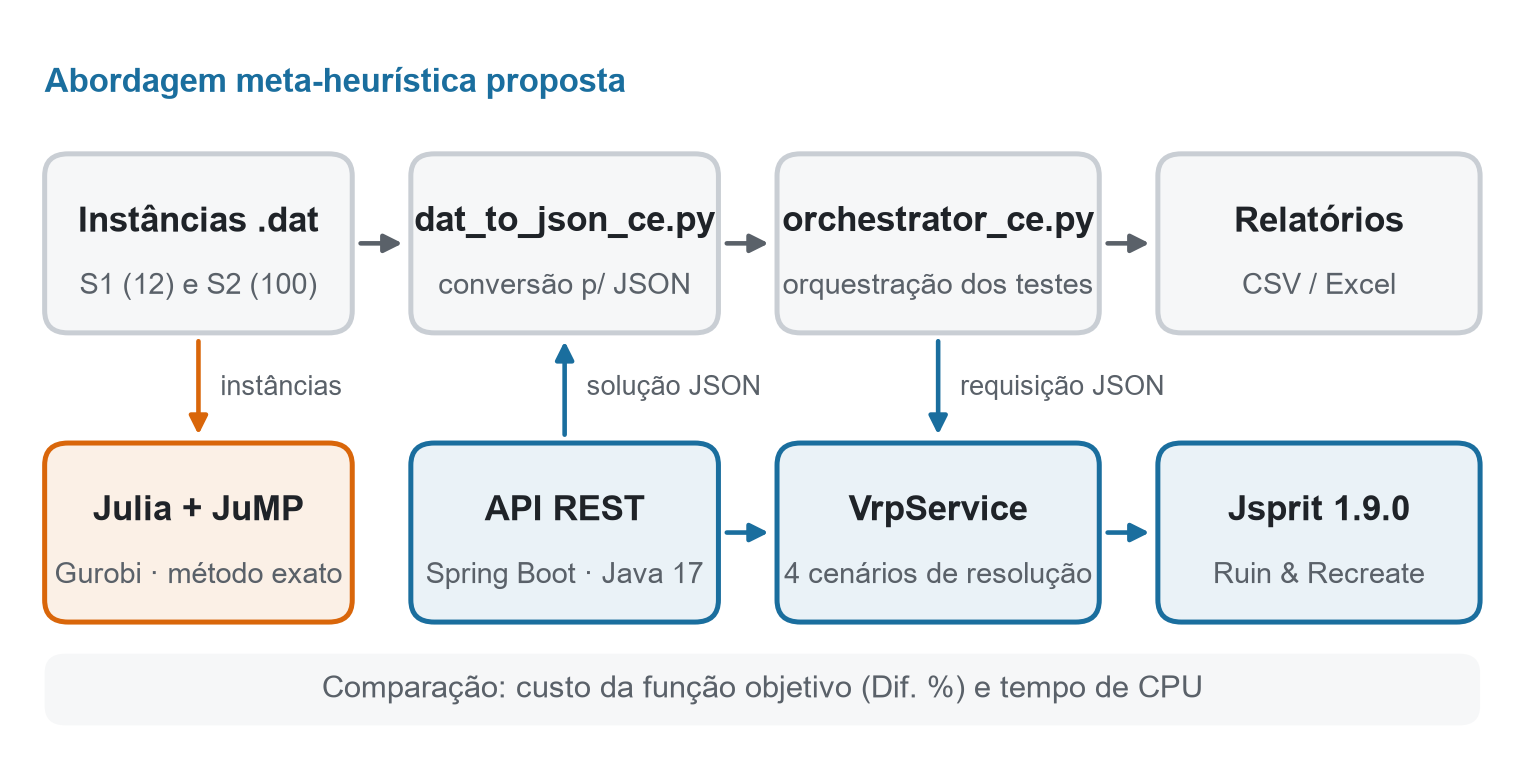
\includegraphics[width=13.5cm]{figuras/fig1_arquitetura.png}
    \caption{Arquitetura do serviço e fluxo experimental}
    \label{fig:1}
\end{figure}

\subsubsection{A meta-heurística \textit{Ruin-and-Recreate}}
O motor de resolução é a biblioteca Jsprit 1.9.0-beta.3, que implementa o esquema \textit{Ruin-and-Recreate} proposto por Schrimpf et al. (2000). O algoritmo parte de uma solução inicial construída por inserção com arrependimento e alterna iterativamente duas fases. Na fase de destruição, um subconjunto dos clientes é removido das rotas, seja pela estratégia radial, que remove clientes próximos a um ponto de referência sorteado, seja pela estratégia aleatória. Na fase de reconstrução, os clientes removidos são reinseridos pela heurística de melhor inserção, que testa todas as posições factíveis e escolhe a de menor acréscimo de custo, ou pela inserção com arrependimento, que prioriza o cliente cuja segunda melhor posição é sensivelmente pior que a melhor, reduzindo o risco de inserções míopes.

A solução resultante de cada iteração é submetida a um critério de aceitação do tipo \textit{Threshold Accepting}, variante determinística do recozimento simulado, que admite pioras limitadas por um limiar decrescente ao longo da execução. Para mitigar a convergência para mínimos locais, adotou-se uma estratégia de múltiplos pontos de partida com sementes determinísticas: cada partida reinstancia o algoritmo e executa mil iterações internas, retendo-se ao final a melhor solução encontrada. A Figura~\ref{fig:2} esquematiza o procedimento e a Tabela~\ref{tab:1} consolida os parâmetros efetivamente empregados.

\begin{figure}[H]
    \centering
    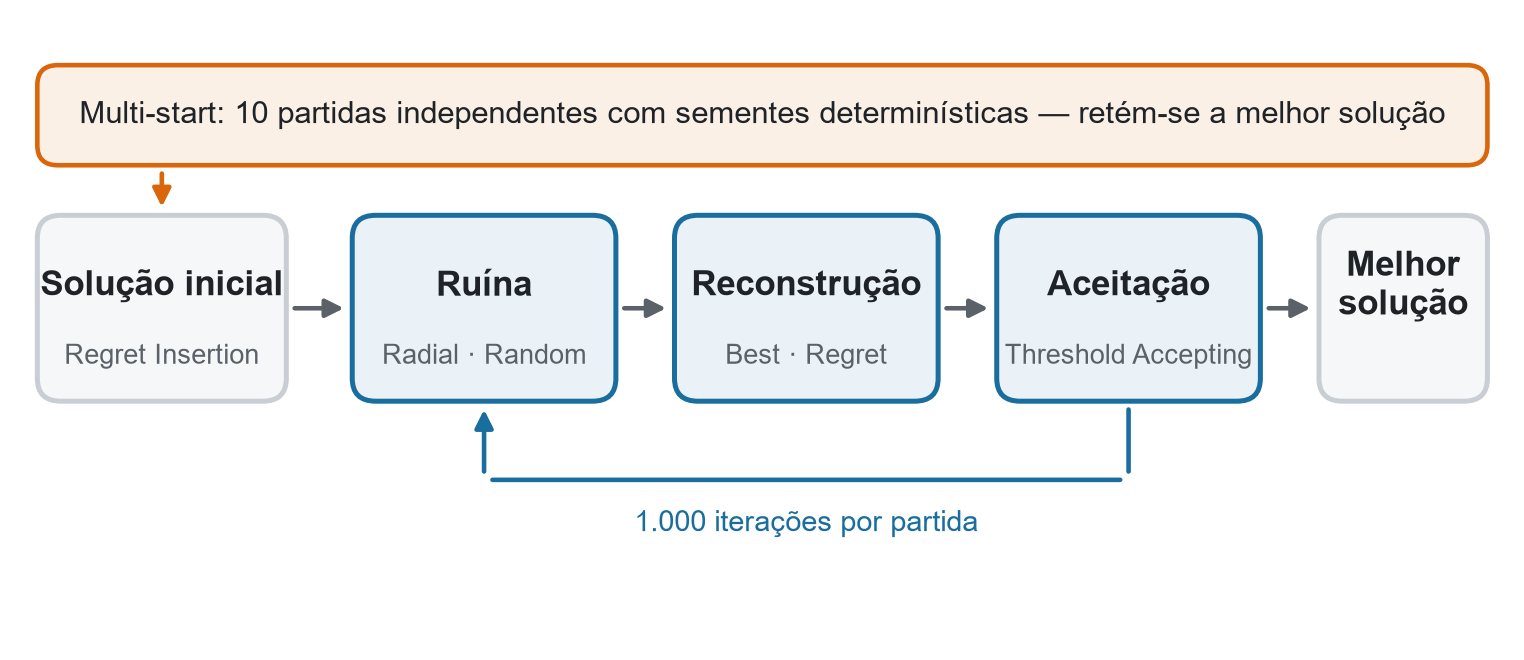
\includegraphics[width=13.5cm]{figuras/fig2_ruin_recreate.png}
    \caption{Esquema do algoritmo \textit{Ruin-and-Recreate} com múltiplas partidas}
    \label{fig:2}
\end{figure}

\begin{table}[H]
    \centering
    \caption{Parâmetros da meta-heurística por modo de resolução}
    \label{tab:1}
    \vspace{0.2cm}
    \footnotesize
    \setlength{\tabcolsep}{4pt}
    \begin{adjustbox}{max width=\textwidth}
    \begin{tabular}{>{\raggedright\arraybackslash}p{4.6cm} c c}
        \toprule
        \textbf{Parâmetro} & \textbf{Com simultaneidade} & \textbf{Sem simultaneidade} \\
        \midrule
        Mecanismo de colaboração & \textit{skills} do Jsprit & alocação enumerada + \textit{SameVehicleConstraint} \\
        Partidas (\textit{multi-start}) & 10 & 2 por alocação, até 7 alocações \\
        Esforço total (iterações) & 10.000 & até 14.000 \\
        Troca de veículo & habilitada & desabilitada \\
        Iterações por partida & \multicolumn{2}{c}{1.000} \\
        Threads & \multicolumn{2}{c}{4} \\
        Limiar inicial ($\theta_0$) & \multicolumn{2}{c}{0,03} \\
        Decaimento do limiar ($\alpha$) & \multicolumn{2}{c}{0,15} \\
        Semente aleatória & \multicolumn{2}{c}{determinística (partida $\times$ 1.000 + 42)} \\
        Tamanho da frota & \multicolumn{2}{c}{finita, máx(n, 20) veículos por transportadora} \\
        \bottomrule
    \end{tabular}
    \end{adjustbox}
\end{table}

\subsubsection{Tradução das restrições para o Jsprit}
A principal dificuldade metodológica do trabalho consistiu em traduzir restrições formuladas de modo declarativo, por meio de inequações, para o paradigma orientado a objetos do Jsprit, no qual elas devem ser expressas por classes de estado e funções de atualização executadas a cada modificação de rota.

As demandas de coleta e entrega de cada cliente foram modeladas como duas tarefas distintas: uma de entrega, que reduz a carga do veículo, e uma de coleta, que a aumenta. Essa separação é necessária para que a verificação de capacidade seja feita corretamente em cada ponto da rota, respeitando a carga acumulada ao longo do trajeto. Para garantir que ambas as tarefas de um mesmo cliente sejam atendidas pelo mesmo veículo físico, exigência que o Jsprit não oferece nativamente para tarefas independentes, implementou-se uma restrição customizada de rota rígida, denominada \textit{SameVehicleConstraint}, apoiada em um atualizador de estado que rastreia, a cada modificação, qual instância de veículo atende cada tarefa. Como a comparação é feita por identidade de objeto, foi necessário declarar a frota com tamanho finito, pré-instanciando um número fixo de veículos por transportadora, de modo que cada rota física corresponda a um objeto distinto.

A colaboração horizontal foi modelada por dois mecanismos, conforme o cenário. No cenário com simultaneidade, empregou-se o mecanismo nativo de habilidades do Jsprit: cada veículo recebe a habilidade correspondente à sua transportadora e cada cliente exclusivo exige a habilidade do seu atendente, ao passo que clientes compartilhados não recebem exigência alguma, delegando ao algoritmo a decisão de alocação. No cenário sem simultaneidade, em que um mesmo cliente pode ser visitado mais de uma vez, o espaço de alocações é explorado externamente: geram-se até sete configurações distintas de atribuição dos clientes compartilhados (todas para a primeira transportadora, todas para a segunda, por proximidade do depósito, por proximidade inversa e variações combinatórias ou aleatórias com semente fixa) e cada configuração é resolvida por uma execução independente da meta-heurística, retendo-se a de menor custo total.

\subsubsection{Instâncias e protocolo experimental}
Os experimentos empregaram os dois conjuntos de instâncias utilizados por Fernández, Roca-Riu e Speranza (2018), adaptados com a inclusão de demandas de coleta. O conjunto S1 reúne 12 instâncias com 18 a 30 clientes. O conjunto S2 reúne 100 instâncias, sendo 50 com clientes distribuídos aleatoriamente em um quadrado de 100 unidades de lado (subconjunto S2R) e 50 com clientes agrupados em três a cinco aglomerados (subconjunto S2C); em cada subconjunto há 10 instâncias para cada porte de 10, 15, 20, 25 e 30 clientes. As demandas de coleta foram geradas de modo que sua soma, por transportadora, igualasse a soma das entregas, preservando a coerência do problema original e evitando alterações na capacidade dos veículos.

Cada instância foi resolvida nos quatro cenários implementados, totalizando 448 execuções da meta-heurística. Destas, 336, correspondentes às três configurações para as quais o método exato dispõe de rotina de resolução equivalente, possuem solução de referência e constituem o objeto da análise que se segue. As execuções ocorreram em processador Intel Core i7 de 3,20 GHz com 16 GB de memória RAM, mesma configuração empregada nas execuções do método exato, o que torna diretamente comparáveis os tempos reportados. Ao otimizador Gurobi foi imposto limite de 7.200 segundos por execução; à meta-heurística não se impôs limite de tempo, sendo o critério de parada exclusivamente o número de iterações.

A métrica de qualidade adotada é a diferença percentual entre o custo obtido pela meta-heurística e o custo obtido pelo método exato, calculada instância a instância. Valores positivos indicam solução mais cara que a de referência; valores negativos indicam que a meta-heurística encontrou solução melhor que o incumbente do otimizador, situação possível quando este encerra a execução por limite de tempo sem comprovar otimalidade. A métrica de eficiência é o tempo de processamento, reportado em segundos e agregado pela média dos grupos.

\subsection{Resultados e Análise}
\label{sec:resultados}
Esta seção apresenta os resultados das 336 execuções comparadas. A apresentação segue a ordem: validação no conjunto reduzido, escalabilidade no conjunto ampliado, efeito da distribuição espacial dos clientes, comportamento nos demais cenários, economia proporcionada pela colaboração e, por fim, discussão das limitações identificadas.

\subsubsection{Validação no conjunto S1}
A Tabela~\ref{tab:2} apresenta, para cada uma das 12 instâncias do conjunto S1, os resultados do método exato e da meta-heurística no cenário completo do problema, com simultaneidade e com colaboração.

\begin{table}[H]
    \centering
    \caption{Conjunto S1: método exato (Gurobi) e meta-heurística (Jsprit) no cenário com simultaneidade e colaboração}
    \label{tab:2}
    \vspace{0.2cm}
    \footnotesize
    \setlength{\tabcolsep}{4pt}
    \begin{adjustbox}{max width=\textwidth}
    \begin{tabular}{c c | c c c | c c | c}
        \toprule
         &  & \multicolumn{3}{c|}{\textbf{Gurobi -- método exato}} & \multicolumn{2}{c|}{\textbf{Jsprit -- meta-heurística}} &  \\
        \textbf{Inst.} & \textbf{Clientes} & \textbf{Custo} & \textbf{Status} & \textbf{CPU (s)} & \textbf{Custo} & \textbf{CPU (s)} & \textbf{Dif. (\%)} \\
        \midrule
        1 & 23 & 279,01 & Ótimo & 966,4 & 282,76 & 34,1 & +1,34 \\
        2 & 29 & 335,82 & Lim. tempo & 7.203,4 & 344,86 & 66,3 & +2,69 \\
        3 & 20 & 238,99 & Ótimo & 357,9 & 239,10 & 35,5 & +0,05 \\
        4 & 23 & 322,30 & Lim. tempo & 7.201,0 & 322,30 & 40,1 & 0,00 \\
        5 & 24 & 331,93 & Ótimo & 3.537,7 & 331,93 & 41,0 & 0,00 \\
        6 & 21 & 230,08 & Ótimo & 18,9 & 230,08 & 41,8 & 0,00 \\
        7 & 20 & 156,93 & Ótimo & 57,2 & 156,93 & 38,0 & 0,00 \\
        8 & 30 & 248,10 & Lim. tempo & 7.201,0 & 243,60 & 76,9 & -1,81 \\
        9 & 20 & 392,06 & Ótimo & 6,6 & 392,06 & 32,8 & 0,00 \\
        10 & 20 & 455,74 & Ótimo & 27,1 & 455,73 & 33,9 & 0,00 \\
        11 & 18 & 499,42 & Ótimo & 12,4 & 499,42 & 24,1 & 0,00 \\
        12 & 20 & 755,37 & Ótimo & 943,5 & 757,76 & 28,7 & +0,32 \\
        Média &  &  &  & 2.294,4 &  & 41,1 & +0,22 \\
        \bottomrule
    \end{tabular}
    \end{adjustbox}
\end{table}

\noindent{\footnotesize \textit{Nota: Dif. (\%) = (custo Jsprit -- custo Gurobi) / custo Gurobi.}}

A diferença percentual média foi de +0,22\%. Em seis instâncias a meta-heurística reproduziu exatamente o custo ótimo e, na instância 10, a diferença limitou-se a uma centésima de unidade de custo, em favor do Jsprit. O resultado mais expressivo ocorreu na instância 8, cujo processamento exato foi interrompido por limite de tempo com 1,79\% de \textit{gap} em aberto: a meta-heurística obteve custo de 243,60 contra 248,10 do incumbente, uma redução de 1,81\%. O pior desempenho relativo ocorreu na instância 2, com desvio de +2,69\%, também ela encerrada por limite de tempo pelo método exato.

Quanto ao tempo, o contraste é expressivo. O método exato consumiu, em média, 2.294,4 segundos por instância, com três execuções encerradas no limite de 7.200 segundos, enquanto a meta-heurística concluiu todas as execuções em média de 41,1 segundos e máximo de 76,9 segundos, o que representa aceleração média de 55,8 vezes, sem limite de tempo imposto.

\subsubsection{Escalabilidade no conjunto S2}
O conjunto S2, com 100 instâncias, permite observar como a diferença de qualidade e o custo computacional evoluem com o porte do problema. A Tabela~\ref{tab:3} consolida os resultados médios por número de clientes.

\begin{table}[H]
    \centering
    \caption{Conjunto S2: resultados médios por número de clientes no cenário com simultaneidade e colaboração}
    \label{tab:3}
    \vspace{0.2cm}
    \footnotesize
    \setlength{\tabcolsep}{4pt}
    \begin{adjustbox}{max width=\textwidth}
    \begin{tabular}{c | c c c | c c | c c}
        \toprule
         & \multicolumn{3}{c|}{\textbf{Gurobi -- método exato}} & \multicolumn{2}{c|}{\textbf{Jsprit -- meta-heurística}} & \multicolumn{2}{c}{\textbf{Comparação}} \\
        \textbf{Clientes} & \textbf{Custo} & \textbf{CPU (s)} & \textbf{Ótimas} & \textbf{Custo} & \textbf{CPU (s)} & \textbf{Dif. (\%)} & \textbf{Acel.} \\
        \midrule
        10 & 474,87 & 2,7 & 20/20 & 474,87 & 11,8 & 0,00 & 0,2$\times$ \\
        15 & 564,39 & 29,5 & 20/20 & 563,91 & 20,9 & -0,05 & 1,4$\times$ \\
        20 & 653,65 & 3.019,5 & 18/20 & 655,17 & 32,3 & +0,22 & 93,5$\times$ \\
        25 & 770,06 & 4.308,4 & 9/20 & 774,21 & 48,3 & +0,46 & 89,2$\times$ \\
        30 & 890,45 & 6.542,1 & 2/20 & 901,59 & 67,5 & +1,17 & 96,9$\times$ \\
        Total & --- & 2.780,4 & 69/100 & --- & 36,2 & +0,36 & 76,9$\times$ \\
        \bottomrule
    \end{tabular}
    \end{adjustbox}
\end{table}

\noindent{\footnotesize \textit{Nota: a instância 8090 foi executada sem limite de tempo (39.532,9 s); desconsiderando-a, o tempo médio do grupo de 20 clientes cai para 1.097,7 s, ainda cerca de 34 vezes o tempo do Jsprit.}}

Três padrões emergem dos dados. O primeiro é a degradação controlada da qualidade: a diferença média parte de 0,00\% no grupo de 10 clientes, mantém-se ligeiramente negativa no grupo de 15 clientes, isto é, a meta-heurística foi, em média, marginalmente melhor que o otimizador, e cresce de forma monotônica até +1,17\% no grupo de 30 clientes, permanecendo em +0,36\% na média geral. O segundo é a fidelidade das soluções: em 60 das 100 instâncias o custo obtido coincide exatamente com o do método exato, e em 4 instâncias o supera. O terceiro é a inversão do regime de tempo: para 10 clientes a meta-heurística é mais lenta que o otimizador, situação que se inverte a partir de 15 clientes e se acentua rapidamente, atingindo aceleração de 96,9 vezes no grupo de 30 clientes.

Cabe observar que parte da diferença medida nos grupos maiores não decorre de deficiência da meta-heurística, mas da própria imprecisão da referência: no grupo de 30 clientes apenas 2 das 20 instâncias foram resolvidas até a otimalidade comprovada, de modo que o valor do otimizador é, nas demais, apenas um limite superior. A Figura~\ref{fig:3} ilustra a divergência entre os regimes de crescimento do tempo de processamento.

\begin{figure}[H]
    \centering
    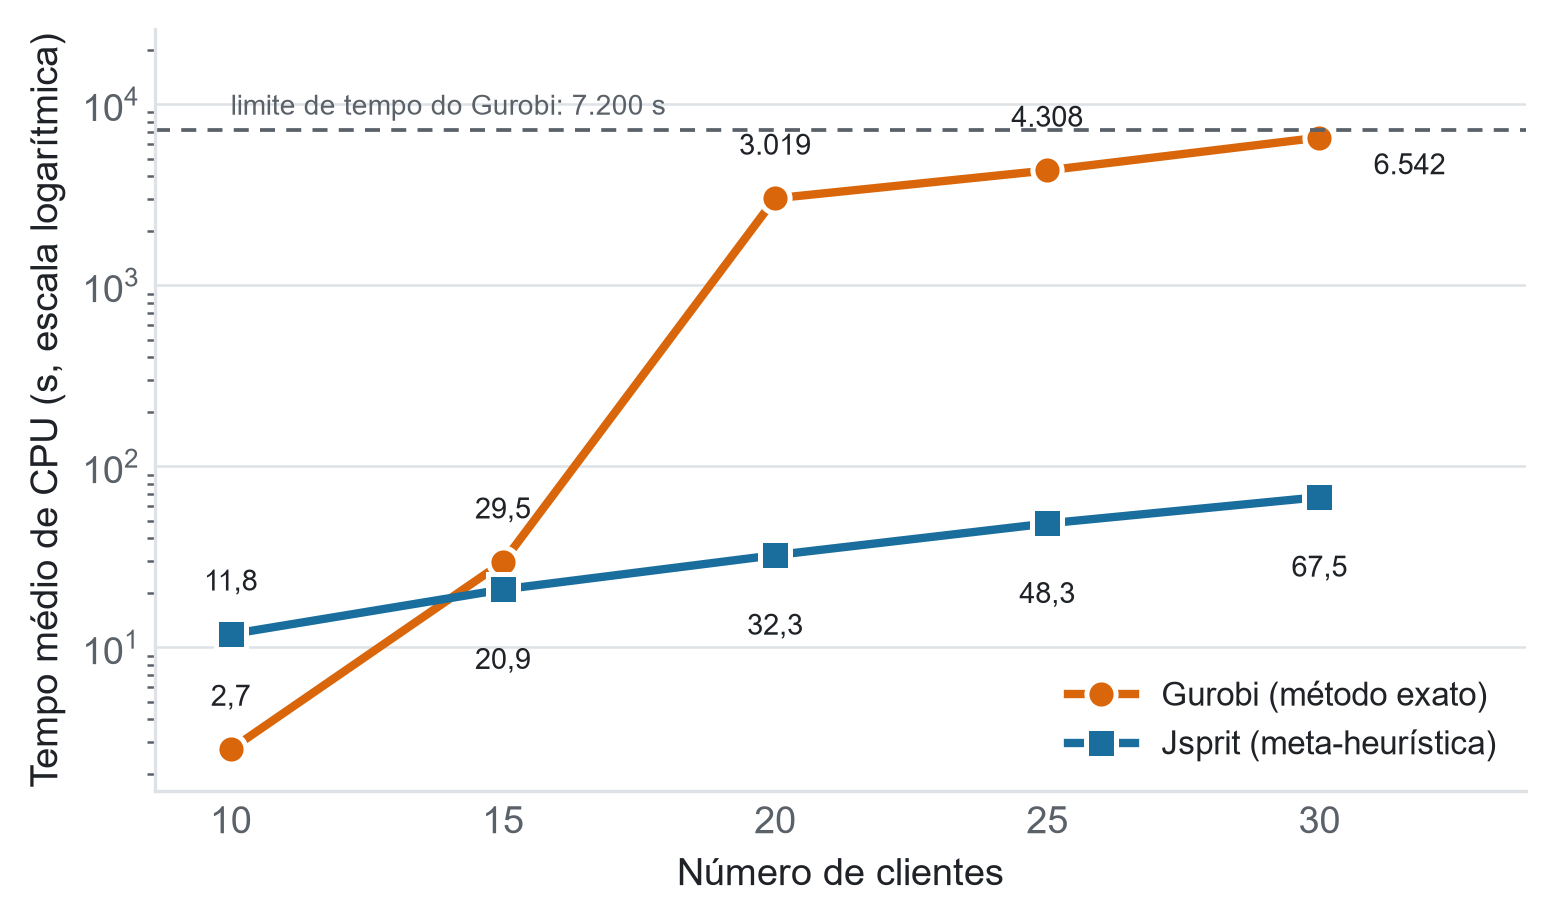
\includegraphics[width=13.5cm]{figuras/fig3_tempo_cpu.png}
    \caption{Tempo médio de processamento por número de clientes (escala logarítmica)}
    \label{fig:3}
\end{figure}

Enquanto o tempo do método exato cresce de forma acentuada, de 2,7 a 6.542,1 segundos, aproximando-se do limite imposto, o tempo da meta-heurística evolui de maneira aproximadamente linear, de 11,8 a 67,5 segundos. Nenhuma execução ultrapassou 82 segundos em todo o conjunto S2, o que situa o serviço na faixa de tempo compatível com uso interativo.

\subsubsection{Efeito da distribuição espacial dos clientes}
O conjunto S2 divide-se em instâncias com clientes dispostos aleatoriamente e instâncias com clientes agrupados em aglomerados. A Tabela~\ref{tab:4} compara o desempenho da meta-heurística nos dois subconjuntos, para os três cenários avaliados.

\begin{table}[H]
    \centering
    \caption{Conjunto S2: desempenho nos subconjuntos aleatório (S2R) e agrupado (S2C)}
    \label{tab:4}
    \vspace{0.2cm}
    \footnotesize
    \setlength{\tabcolsep}{4pt}
    \begin{adjustbox}{max width=\textwidth}
    \begin{tabular}{>{\raggedright\arraybackslash}p{4.2cm} | c c c | c c c}
        \toprule
         & \multicolumn{3}{c|}{\textbf{S2R -- aleatórias (50)}} & \multicolumn{3}{c}{\textbf{S2C -- agrupadas (50)}} \\
        \textbf{Cenário} & \textbf{Dif. (\%)} & \textbf{Iguais} & \textbf{Acel.} & \textbf{Dif. (\%)} & \textbf{Iguais} & \textbf{Acel.} \\
        \midrule
        Com simultaneidade & +0,45 & 30 & 52,9$\times$ & +0,27 & 30 & 101,6$\times$ \\
        Sem simultaneidade & +2,52 & 17 & 55,4$\times$ & +3,63 & 17 & 55,7$\times$ \\
        Sem compartilhamento & +0,14 & 41 & 63,9$\times$ & +0,17 & 35 & 113,7$\times$ \\
        \bottomrule
    \end{tabular}
    \end{adjustbox}
\end{table}

\noindent{\footnotesize \textit{Nota: ``Iguais'' indica o número de instâncias em que o Jsprit reproduziu exatamente o custo do método exato. Os valores do cenário sem simultaneidade refletem a limitação de modelagem discutida na seção de resultados.}}

No cenário completo, a meta-heurística apresenta desempenho relativo superior nas instâncias agrupadas (+0,27\%) em comparação às aleatórias (+0,45\%), ao mesmo tempo em que a aceleração praticamente dobra, passando de 52,9 para 101,6 vezes. O resultado tem explicação direta: a estrutura em aglomerados agrava a dificuldade do método exato, que encerrou por limite de tempo 19 das 50 instâncias agrupadas contra 12 das 50 aleatórias, mas não penaliza de forma equivalente a busca local do esquema \textit{Ruin-and-Recreate}, cuja estratégia de destruição radial é particularmente adequada a clientes espacialmente concentrados.

\subsubsection{Cenários sem simultaneidade e sem compartilhamento}
A Tabela~\ref{tab:5} e a Figura~\ref{fig:4} comparam o comportamento da meta-heurística nos três cenários avaliados sobre o conjunto S2.

\begin{table}[H]
    \centering
    \caption{Diferença percentual média por cenário e por número de clientes (conjunto S2)}
    \label{tab:5}
    \vspace{0.2cm}
    \footnotesize
    \setlength{\tabcolsep}{4pt}
    \begin{adjustbox}{max width=\textwidth}
    \begin{tabular}{>{\raggedright\arraybackslash}p{5.0cm} c c c c c c c}
        \toprule
        \textbf{Cenário} & \textbf{10 cli.} & \textbf{15 cli.} & \textbf{20 cli.} & \textbf{25 cli.} & \textbf{30 cli.} & \textbf{Média} & \textbf{Iguais} \\
        \midrule
        Com simultaneidade (colaborativo) & 0,00 & -0,05 & +0,22 & +0,46 & +1,17 & +0,36 & 60/100 \\
        Sem simultaneidade (colaborativo) & +0,48 & +1,21 & +3,30 & +3,28 & +7,10 & +3,07 & 34/100 \\
        Sem compartilhamento & 0,00 & 0,00 & +0,22 & +0,13 & +0,42 & +0,16 & 76/100 \\
        \bottomrule
    \end{tabular}
    \end{adjustbox}
\end{table}

\begin{figure}[H]
    \centering
    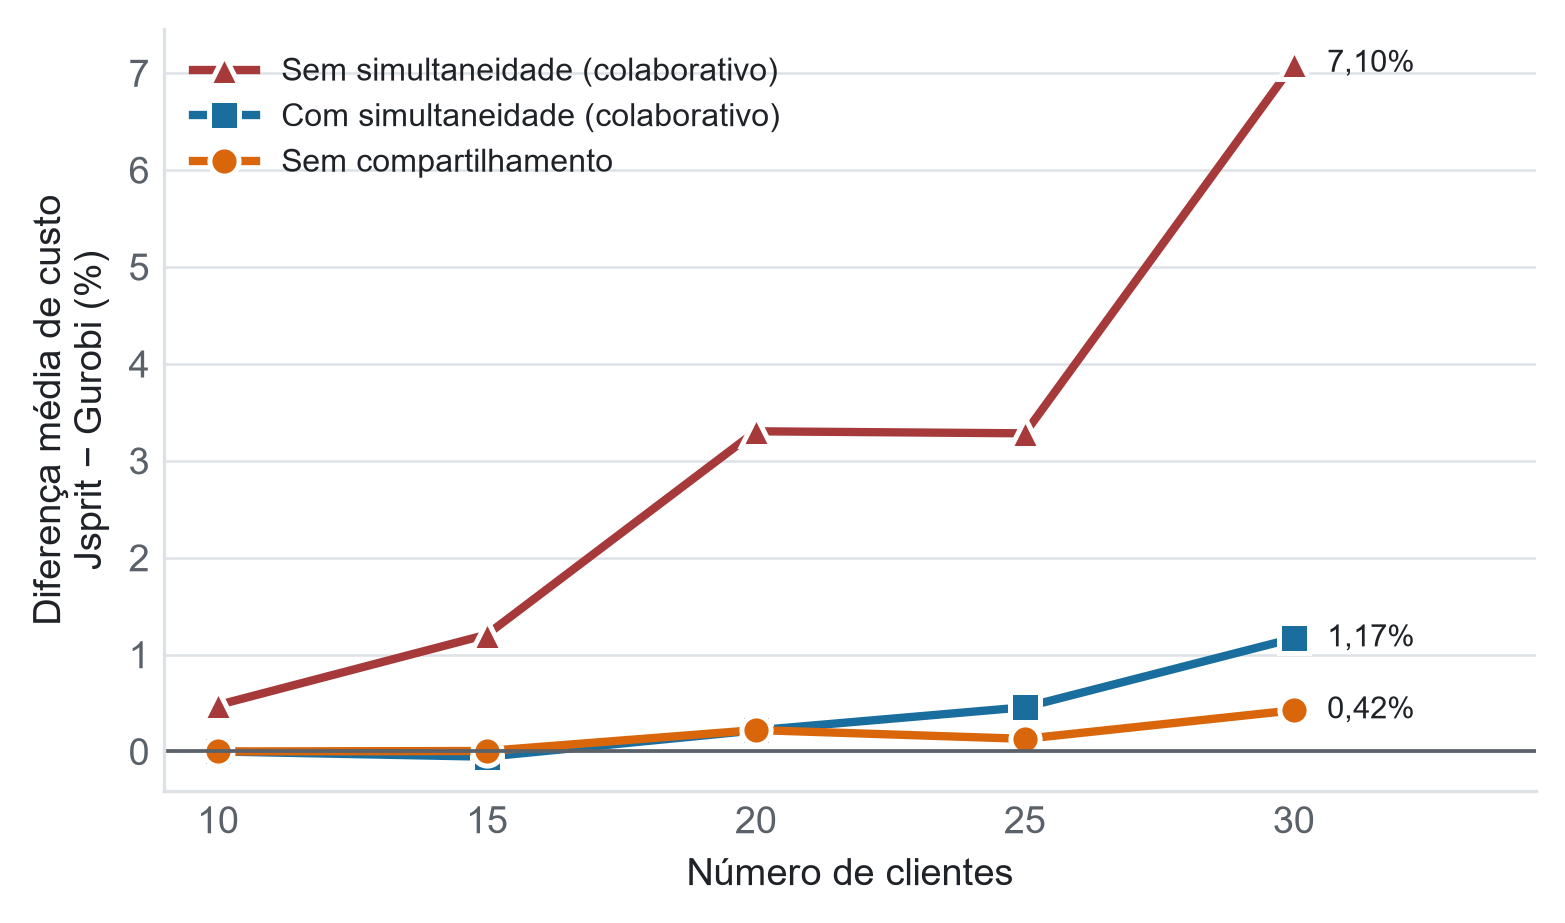
\includegraphics[width=13.5cm]{figuras/fig4_desvio_custo.png}
    \caption{Diferença média de custo por cenário e número de clientes}
    \label{fig:4}
\end{figure}

O cenário sem compartilhamento é aquele em que a meta-heurística mais se aproxima da referência, com diferença média de apenas +0,16\% e reprodução exata do ótimo em 76 das 100 instâncias. O resultado é coerente com a natureza do cenário: sem colaboração, o problema se decompõe em dois subproblemas independentes e substancialmente menores, cujo espaço de busca é mais facilmente varrido. Esse cenário funciona, portanto, como verificação de sanidade da implementação, atestando que os desvios observados nos demais casos decorrem da dificuldade do problema colaborativo e não de erro de modelagem.

O cenário sem simultaneidade, ao contrário, é o mais desafiador: a diferença média sobe para +3,07\% no conjunto S2 e +3,85\% no conjunto S1, com degradação acentuada nos grupos maiores, chegando a +7,10\% para 30 clientes. Em nenhuma instância a meta-heurística superou o método exato.

A investigação dessa diferença conduziu a uma auditoria das rotas produzidas, cujo resultado altera a interpretação dos números. Nas 112 instâncias resolvidas no cenário sem simultaneidade, nenhum cliente foi atendido por duas transportadoras e nenhum cliente recebeu mais de uma visita. A mesma verificação aplicada às soluções do método exato no mesmo cenário mostra o oposto: em seis das oito instâncias cujas rotas foram preservadas há ao menos um cliente atendido pelas duas transportadoras e, em cinco delas, ao menos um cliente visitado duas vezes pela mesma transportadora. Aplicado às soluções do cenário com simultaneidade, o procedimento retorna zero para ambos os métodos, como esperado, o que atesta sua validade.

A causa está na modelagem adotada. Para um cliente compartilhado, as demandas das duas transportadoras são somadas em um único par de tarefas de entrega e coleta, ao qual se associa a habilidade da transportadora definida na etapa de alocação. Esse cliente resulta, portanto, sempre atendido uma única vez e por uma única transportadora, que é precisamente o que a restrição de simultaneidade impõe. A possibilidade que caracteriza o cenário relaxado, a de que cada transportadora atenda separadamente a sua própria demanda no mesmo cliente, nunca chega a ser construída.

Disso decorre que a diferença de 3,07\% não mede a dificuldade da meta-heurística diante da variante relaxada. Ela mede a distância entre uma solução do modelo restrito e uma referência obtida no modelo relaxado, que são formulações distintas. O espaço efetivamente percorrido nesse cenário é um subconjunto daquele percorrido no cenário com simultaneidade, com a alocação congelada previamente em vez de decidida pela busca. Isso explica que em nenhuma instância a meta-heurística tenha superado o método exato e que, em 55 das 112 instâncias, ela tenha devolvido solução mais cara do que a obtida por ela própria no cenário restrito, resultado impossível entre soluções ótimas verdadeiras.

Os resultados deste cenário devem ser lidos, portanto, como limitação identificada da implementação, e não como medida de desempenho da meta-heurística na variante sem simultaneidade. Os demais cenários não são afetados: tanto no cenário com simultaneidade quanto no cenário sem compartilhamento as tarefas de um cliente compartilhado não recebem habilidade restritiva, e a escolha da transportadora cabe à própria busca, em conformidade com o modelo correspondente. A correção necessária, detalhada entre os desdobramentos, consiste em criar um par de tarefas por transportadora para o cliente compartilhado, dispensando a enumeração externa de configurações, e em substituir a exigência de mesmo veículo pela de mesma transportadora, que é o que o modelo de referência estabelece.

\subsubsection{Economia proporcionada pela colaboração}
O propósito último do modelo colaborativo é quantificar quanto se economiza quando duas transportadoras compartilham clientes, em comparação com a operação independente. A Tabela~\ref{tab:6} e a Figura~\ref{fig:5} apresentam essa economia, calculada tanto a partir das soluções do método exato quanto das soluções da meta-heurística.

\begin{table}[H]
    \centering
    \caption{Economia proporcionada pela colaboração horizontal: método exato e meta-heurística}
    \label{tab:6}
    \vspace{0.2cm}
    \footnotesize
    \setlength{\tabcolsep}{4pt}
    \begin{adjustbox}{max width=\textwidth}
    \begin{tabular}{>{\raggedright\arraybackslash}p{4.5cm} c | c c | c}
        \toprule
         &  & \multicolumn{2}{c|}{\textbf{Economia da colaboração (\%)}} &  \\
        \textbf{Conjunto} & \textbf{Instâncias} & \textbf{Gurobi} & \textbf{Jsprit} & \textbf{Dif. (p.p.)} \\
        \midrule
        S1 (12 instâncias) & 12 & 12,09 & 12,01 & 0,08 \\
        S2 -- 10 clientes & 20 & 7,54 & 7,54 & 0,00 \\
        S2 -- 15 clientes & 20 & 7,72 & 7,78 & 0,06 \\
        S2 -- 20 clientes & 20 & 13,25 & 13,26 & 0,01 \\
        S2 -- 25 clientes & 20 & 9,08 & 8,79 & 0,28 \\
        S2 -- 30 clientes & 20 & 10,80 & 10,14 & 0,66 \\
        S2R -- aleatórias & 50 & 12,00 & 11,74 & 0,26 \\
        S2C -- agrupadas & 50 & 7,35 & 7,26 & 0,09 \\
        S2 -- total & 100 & 9,68 & 9,50 & 0,17 \\
        \bottomrule
    \end{tabular}
    \end{adjustbox}
\end{table}

\noindent{\footnotesize \textit{Nota: economia = (custo sem compartilhamento -- custo colaborativo) / custo sem compartilhamento, calculada instância a instância e depois promediada.}}

\begin{figure}[H]
    \centering
    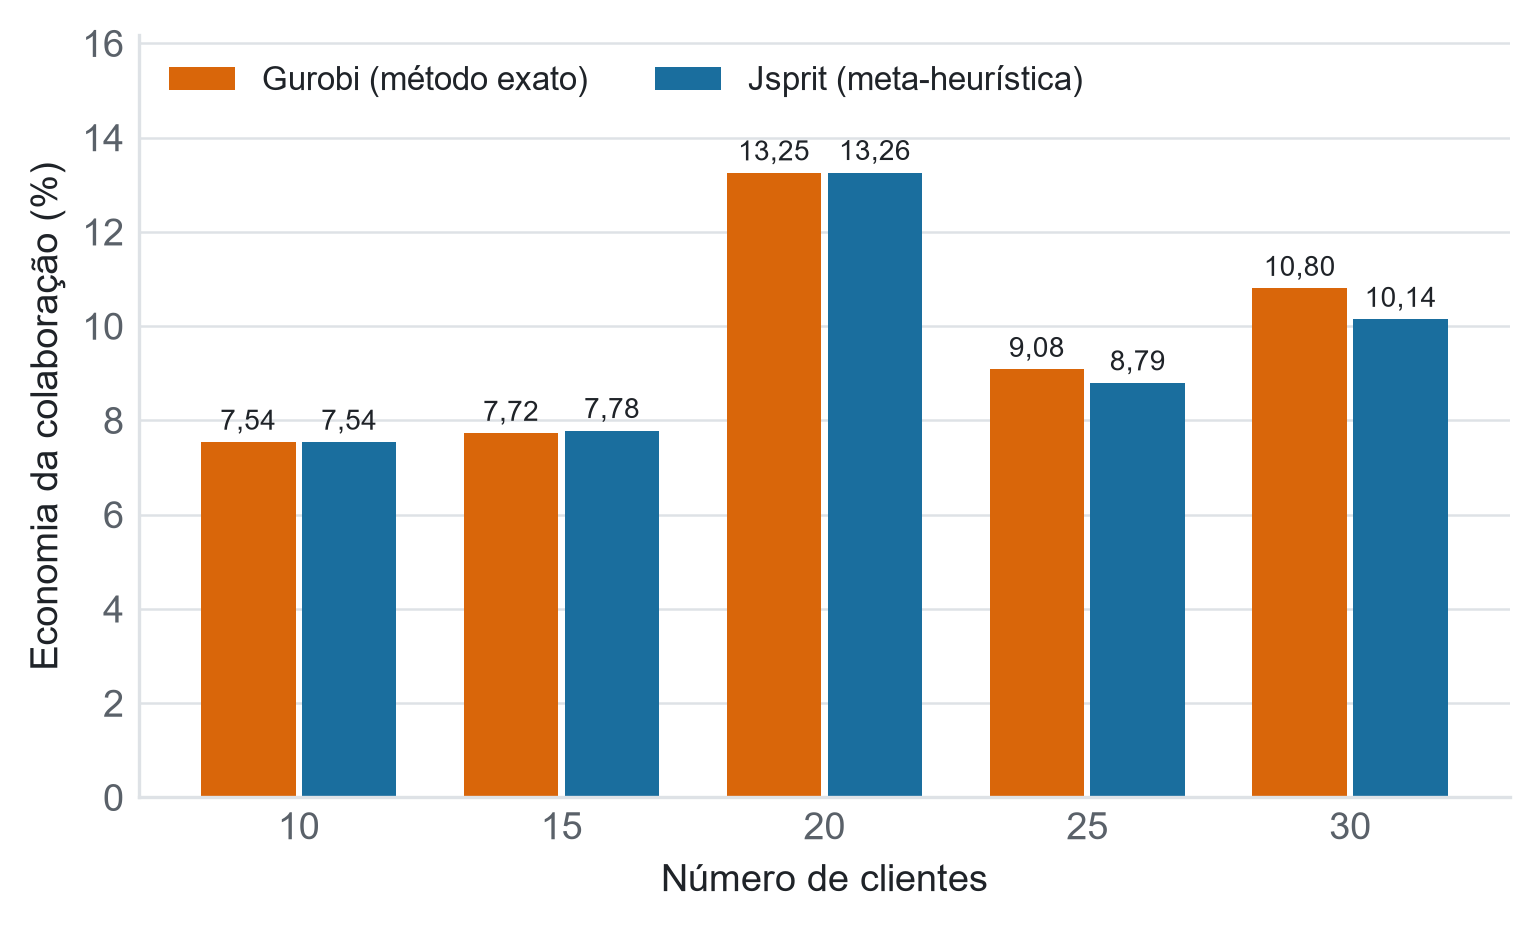
\includegraphics[width=13.5cm]{figuras/fig5_economia_colaboracao.png}
    \caption{Economia da colaboração por grupo de instâncias: método exato e meta-heurística}
    \label{fig:5}
\end{figure}

A colaboração horizontal proporcionou economia média de 9,50\% no conjunto S2 e de 12,01\% no conjunto S1, com máximo de 13,26\% no grupo de 20 clientes. A economia é consistentemente maior nas instâncias aleatórias (11,74\%) do que nas agrupadas (7,26\%), o que se explica pela estrutura do problema: quando os aglomerados contêm clientes exclusivos de ambas as transportadoras, transferir os clientes compartilhados de uma para a outra não evita que ambas visitem o mesmo aglomerado, e o ganho da colaboração se reduz.

O resultado de maior relevância prática, porém, está na última coluna da Tabela~\ref{tab:6}. A estimativa de economia produzida pela meta-heurística difere da obtida pelo método exato em, no máximo, 0,66 ponto percentual, e em apenas 0,17 ponto percentual na média do conjunto S2. Isso significa que os erros cometidos pela meta-heurística nos dois cenários comparados são de magnitude semelhante e, portanto, cancelam-se em larga medida na razão que define a economia. A consequência é direta: para responder à pergunta gerencial ``compensa colaborar, e quanto se ganha com isso?'', o serviço desenvolvido fornece, em dezenas de segundos, praticamente a mesma resposta que o método exato forneceria em horas.

As Figuras~\ref{fig:6} e~\ref{fig:7} ilustram graficamente o efeito da colaboração sobre as rotas da instância 1, contrastando a operação independente com a operação colaborativa. Os depósitos das duas transportadoras estão assinalados por quadrados e os clientes por círculos; as cores indicam a transportadora responsável e os clientes compartilhados são representados pelas duas cores. Na operação independente, ambas as transportadoras percorrem os mesmos clientes compartilhados; na operação colaborativa, cada um deles é atendido por uma única transportadora, e as rotas se reorganizam de modo a encurtar o percurso agregado.

\begin{figure}[H]
    \centering
    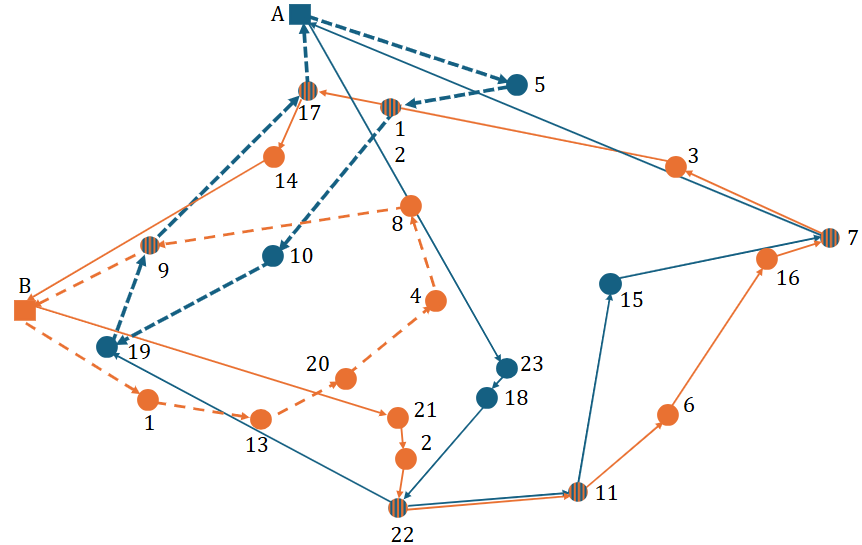
\includegraphics[width=11.5cm]{figuras/artigo_Im3.png}
    \caption{Rotas da instância 1 sem colaboração (custo total 341,89)}
    \label{fig:6}
\end{figure}

\begin{figure}[H]
    \centering
    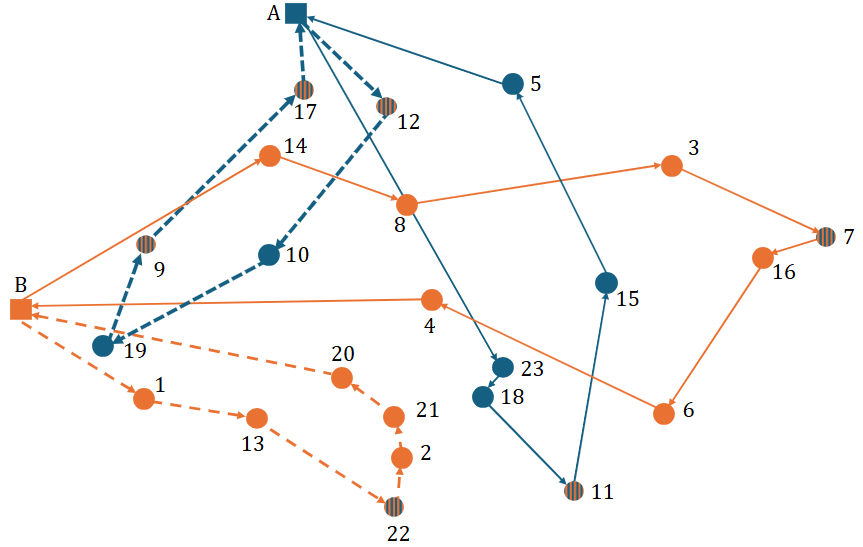
\includegraphics[width=11.5cm]{figuras/artigo_Im4.png}
    \caption{Rotas da instância 1 com colaboração (custo total 279,01)}
    \label{fig:7}
\end{figure}

\noindent{\footnotesize \textit{Nota: rotas obtidas pelo método exato. No cenário sem colaboração a meta-heurística reproduziu exatamente o custo de 341,89; no cenário colaborativo obteve 282,76, correspondente a desvio de 1,34\%.}}

\subsubsection{Limitações e diferenças estruturais}
Apesar do esforço de espelhar fielmente o modelo matemático no \textit{framework} Jsprit, subsistem diferenças estruturais que explicam os desvios observados e delimitam o alcance das conclusões. A mais evidente é de natureza: o otimizador exato retorna provas de otimalidade ou limites válidos, ao passo que a meta-heurística não oferece garantia alguma sobre a distância ao ótimo: as diferenças aqui reportadas são medidas empíricas, não cotas.

A segunda diferença é de representação. O modelo exato emprega variáveis contínuas de fluxo que descrevem explicitamente a carga destinada a cada cliente em cada arco, enquanto o Jsprit rastreia apenas a carga agregada do veículo. A terceira, e mais consequente, diz respeito à alocação dos clientes compartilhados: no modelo exato essa decisão é endógena, e o otimizador explora simultaneamente todas as atribuições possíveis; no serviço desenvolvido ela é tratada pelo mecanismo de habilidades ou por enumeração externa de configurações, o que pode não cobrir todas as combinações quando o número de clientes compartilhados é elevado. No cenário sem simultaneidade essa diferença deixa de ser de grau e passa a ser de natureza, conforme a auditoria relatada na seção anterior.

Por fim, a comparação de tempos deve ser lida com a devida cautela. Embora ambos os métodos tenham sido executados na mesma configuração de hardware, o otimizador operou sob limite de 7.200 segundos, o que trunca seus tempos nas instâncias mais difíceis e, portanto, subestima a aceleração real da meta-heurística nesses casos. Em uma instância do grupo de 20 clientes, executada sem limite de tempo, o método exato consumiu 39.532,9 segundos, cerca de onze horas, contra 29,9 segundos da meta-heurística.

\section{Conclusão}
Este trabalho desenvolveu e validou um serviço web para a resolução do problema de roteamento de veículos colaborativo com clientes compartilhados e coletas e entregas simultâneas. Foram implementados, sobre a biblioteca Jsprit, os quatro cenários do problema, o que exigiu traduzir para o paradigma orientado a objetos restrições originalmente formuladas de modo declarativo, notadamente o vínculo entre as tarefas de coleta e entrega de um mesmo cliente e o controle da alocação dos clientes compartilhados. A validação percorreu 112 instâncias em quatro cenários, totalizando 448 execuções comparadas com os resultados do método exato.

Os resultados sustentam três conclusões principais. A primeira é que a meta-heurística aproxima o ótimo com fidelidade elevada no cenário completo do problema: diferença média de 0,22\% no conjunto S1 e de 0,36\% no conjunto S2, com reprodução exata do custo ótimo em 60 das 100 instâncias do conjunto ampliado e soluções superiores ao incumbente do otimizador em instâncias que este não resolveu até a otimalidade. A segunda é que o ganho computacional é de ordem de grandeza: nenhuma execução ultrapassou 82 segundos, contra médias superiores a 6.500 segundos do método exato nas maiores instâncias, com aceleração de até 96,9 vezes. Esses dois resultados, em conjunto, respondem afirmativamente à questão que motivou a pesquisa: é possível obter, em tempo compatível com uso interativo, soluções cuja distância ao ótimo não altera materialmente a decisão logística.

A terceira conclusão é a de maior interesse aplicado. A economia proporcionada pela colaboração horizontal, estimada em 9,50\% em média no conjunto S2, é reproduzida pela meta-heurística com desvio inferior a 0,2 ponto percentual em relação ao método exato. Como os erros da meta-heurística nos cenários colaborativo e independente têm magnitude semelhante e se cancelam na razão que define a economia, o serviço desenvolvido pode ser empregado com segurança para dimensionar o benefício de uma coalizão entre transportadoras, sem depender da disponibilidade de um otimizador comercial nem de horas de processamento.

O trabalho também delimitou onde a abordagem falha, e o fez por auditoria das próprias soluções. No cenário sem a restrição de simultaneidade, nenhuma das 112 instâncias produziu cliente atendido por duas transportadoras, ao passo que o método exato produz esse padrão em seis das oito instâncias verificadas. A implementação soma as demandas das duas transportadoras em um único par de tarefas e, com isso, nunca constrói a possibilidade que define esse cenário. A diferença de 3,07\% ali reportada mede, portanto, uma lacuna de modelagem, e não o desempenho da meta-heurística na variante relaxada. Os demais cenários, que sustentam as conclusões anteriores, não são afetados.

Como desdobramentos, apontam-se quatro direções. A primeira é a implementação da variante muitos-para-muitos, na qual se elimina a figura do depósito central único e as demandas passam a ser expressas como pares origem-destino distribuídos arbitrariamente na rede. Trata-se de variante inicialmente prevista neste ciclo, cujo mapeamento das estruturas de dados foi iniciado, mas que não produziu resultados experimentais em tempo hábil e permanece, portanto, como trabalho futuro. A segunda, de execução imediata, é a correção da modelagem do cenário sem simultaneidade, criando um par de tarefas por transportadora para o cliente compartilhado, substituindo a exigência de mesmo veículo pela de mesma transportadora e reexecutando os dois conjuntos de instâncias, de modo a obter para esse cenário medida comparável à dos demais. A terceira é a adoção de estratégias de partida quente, inicializando a busca a partir de soluções construtivas de boa qualidade. A quarta é a extensão do modelo a janelas de tempo e frotas heterogêneas, ampliando sua aderência a contextos logísticos reais.

\section*{Referências Bibliográficas}
\begin{thebibliography}{99}
\addcontentsline{toc}{section}{Referências}
\bibitem{ref1} CACERES-CRUZ, J. et al. Rich vehicle routing problem: survey. ACM Computing Surveys, v. 47, n. 2, 2014.
\bibitem{ref2} CORDEAU, J.-F.; LAPORTE, G.; ROPKE, S. Recent models and algorithms for one-to-one pickup and delivery problems. In: GOLDEN, B.; RAGHAVAN, S.; WASIL, E. (ed.). The \textit{Vehicle Routing Problem}: latest advances and new challenges. Boston: Springer, 2008. p. 327-357.
\bibitem{ref3} FERNÁNDEZ, E.; ROCA-RIU, M.; SPERANZA, M. G. The shared customer collaboration vehicle routing problem. \textit{European Journal of Operational Research}, v. 265, n. 3, p. 1078-1093, 2018.
\bibitem{ref4} GANSTERER, M.; HARTL, R. F. Collaborative vehicle routing: a survey. \textit{European Journal of Operational Research}, v. 268, n. 1, p. 1-12, 2018.
\bibitem{ref5} GANSTERER, M.; HARTL, R. F. Shared resources in collaborative vehicle routing. TOP, v. 28, n. 1, p. 1-20, 2020.
\bibitem{ref6} GRAPHHOPPER. jsprit: java based, open source toolkit for solving rich vehicle routing problems. Versão 1.9.0-beta.3. Disponível em: https://github.com/graphhopper/jsprit. Acesso em: 20 jul. 2026.
\bibitem{ref7} GUROBI OPTIMIZATION. Gurobi Optimizer Reference Manual. Beaverton: Gurobi Optimization, 2024.
\bibitem{ref8} HIMSTEDT, B.; MEISEL, F. A systematic evaluation of extensions for the shared customer collaboration vehicle routing problem. Bremen: Bundesvereinigung Logistik (BVL), 2021.
\bibitem{ref9} PADMANABHAN, B. et al. Potential benefits of carrier collaboration in vehicle routing problem with pickup and delivery. Transportation Letters, v. 14, n. 3, p. 258-273, 2022.
\bibitem{ref10} PAN, S. et al. Horizontal collaborative transport: survey of solutions and practical implementation issues. International Journal of Production Research, v. 57, n. 15-16, p. 5340-5361, 2019.
\bibitem{ref11} PLOSKAS, N. et al. A tangible collaborative decision support system for various variants of the vehicle routing problem. Lecture Notes in Business Information Processing, v. 216, p. 73-84, 2015.
\bibitem{ref12} RAN, L.; LI, L.; ZHAO, X. Brief review on heterogeneous vehicle routing problems. In: IEEE CHINESE CONTROL AND DECISION CONFERENCE. Anais [...]. IEEE, 2022. p. 5847-5852.
\bibitem{ref13} SCHRIMPF, G. et al. Record breaking optimization results using the ruin and recreate principle. Journal of Computational Physics, v. 159, n. 2, p. 139-171, 2000.
\bibitem{ref14} TORRES-RAMOS, A. F. et al. A GRASPxILS for the shared customer collaboration vehicle routing problem. IFAC-PapersOnLine, v. 52, n. 13, p. 2608-2613, 2019.
\bibitem{ref15} VERDONCK, L. et al. Collaborative logistics from the perspective of road transportation companies. Transport Reviews, v. 33, n. 6, p. 700-719, 2013.
\bibitem{ref16} WANG, Y. et al. Collaboration and transportation resource sharing in multiple centers vehicle routing optimization with delivery and pickup. Knowledge-Based Systems, v. 160, p. 296-310, 2018.
\bibitem{ref17} ZHANG, W. et al. Composite multi-objective optimization on a new collaborative vehicle routing problem with shared carriers and depots. Journal of Cleaner Production, v. 274, 2020.
\end{thebibliography}

\end{document}
